\documentclass[dvipdfmx,runningheads]{llncs}
\setcounter{tocdepth}{3}
\usepackage{amssymb}
\usepackage{here}
\usepackage{enumitem}
\usepackage{algorithm}
\usepackage{algorithmic}
\usepackage{wrapfig}
\usepackage{tikz}
\usepackage{amsmath}
\usepackage{docmute}
\usetikzlibrary{automata}
\usetikzlibrary{arrows}
\usetikzlibrary{positioning}
\usetikzlibrary{lindenmayersystems}

\usetikzlibrary{decorations.markings}
\DeclareMathOperator*{\argmin}{arg\,min}
\title{Towards the Algorithmic Molecular Self-Assembly of Fractals by Cotranscriptional Folding\thanks{This work is in part supported by JST Program to Disseminate Tenure Tracking System, MEXT, Japan, No.~6F36 and by JSPS KAKENHI Grant-in-Aid for Young Scientists (A) No.~16H05854 to S.~S.}}
\titlerunning{Algorithmic Self-Assembly of Fractals by Cotranscriptional Folding}
\author{
Yusei Masuda \and 
Shinnosuke Seki\thanks{Corresponding author} \and 
Yuki Ubukata
}
\institute{
Department of Computer and Network Engineering, 
The University of Electro-Communications, 
1-5-1, Chofugaoka, Chofu, Tokyo, 1828585, Japan 
\email{s.seki@uec.ac.jp}
}

\begin{document}

\maketitle

\begin{abstract}
RNA cotranscriptional folding has been recently proven capable of self-assembling a rectangular tile \textit{in vitro} (RNA origami). 
The oritatami system is a novel computational model of cotranscriptional folding. 
In this paper, we initiate the theoretical study on the algorithmic self-assembly of shapes by cotranscriptional folding using the oritatami system. 
We propose an oritatami system that folds into an arbitrary finite portion of the Heighway dragon, which is a fractal also-known as the paperfolding sequence $P = {\rm RRLRRLLR} \cdots$. 
The $i$-th element of $P$ can be obtained by feeding $i$ in binary to a 4-state deterministic finite automaton with output (DFAO). 
We implement this DFAO and a bit-sequence bifurcation component as modules of oritatami system. 
Combining them with a known binary counter module yields the proposed oritatami system. 
\end{abstract}


%-------------------------------------------------------------------------------------------
	\section{Introduction}
%-------------------------------------------------------------------------------------------

An RNA sequence, over nucleotides of four kinds {\tt A}, {\tt C}, {\tt G}, {\tt U}, is synthesized (\textit{transcribed}) from its template DNA sequence over {\tt A}, {\tt C}, {\tt G}, {\tt T} nucleotide by nucleotide by an RNA polymerase (RNAP) enzyme according to the one-to-one mapping ${\tt A} \to {\tt U}$, ${\tt C} \to {\tt G}$, ${\tt G} \to {\tt C}$, and ${\tt T} \to {\tt A}$ (for details, see, e.g., \cite{AJLMRRW2014}). 
The yield, called \textit{transcript}, starts folding immediately after it emerges from RNAP. 
This is the \textit{cotranscriptional folding} (see Fig.~\ref{fig:rna_origami}). 
Geary, Rothemund, and Andersen have recently demonstrated the capability of cotranscriptional folding to self-assemble an RNA molecule of an intended shape at nano-scale \cite{GearyRothemundAndersen2014}. 
They actually proposed an architecture of a DNA sequence whose transcript folds cotranscriptionally into an RNA tile of specific rectangular shape highly likely \textit{in vitro}. 

\begin{figure}[tb]
\centering
\includegraphics[width=\linewidth]{pic/rna_origami.pdf}
\caption{RNA cotranscriptional folding. 
An RNA polymerase attaches to a template DNA sequence (gray spiral), scans it through, and synthesizes its RNA copy. 
The RNA sequence begins to fold upon itself immediately as it emerges from polymerase. 
}
\label{fig:rna_origami}
\end{figure}

%In this paper, we shall initiate the theoretical study on algorithmic self-assembly of shapes by cotranscriptional folding using a novel computational model of cotranscriptional folding called the \textit{oritatami system} \cite{GeMeScSe2016}.
Algorithms and computation are fundamental to molecular self-assembly as illustrated in an enormous success of their use in DNA tile self-assembly (see, e.g., \cite{Doty2012,Patitz2016,WinfreePhD} and references therein). 
%The concepts of computation and algorithms are yet to be as much utilized in the self-assembly of shapes by cotranscriptional folding as in the DNA tile self-assembly, where for example 
The Sierpinski triangle fractal was algorithmically self-assembled even \textit{in vitro} from coalescence of DNA tiles that compute XOR \cite{RothemundPapadakisWinfree2004}. 
Cotranscriptional folding exhibits highly sophisticated computational and algorithmic behaviors as well. 
Indeed, fluoride riboswitches in \textit{Bacillus cereus} bacteria cotranscriptionally fold into a terminator stem or does not in order to regulate gene expression \cite{WaStYuLiLu2016}. %depending on ligand concentration \cite{WaStYuLiLu2016}. 
This is just one example but should be enough to signify the context-sensitivity of cotranscriptional folding and shapes thus self-assembled. 
Geary et al.~have proved the capability of context-sensitivity to count in binary using a novel mathematical model of cotranscriptional folding called \textit{oritatami system} \cite{GeMeScSe2016}. 

%Cotranscriptional folding is in fact proved Turing-universal by the oritatami system \cite{GeMeScSe2015}. 
%The Turing-machine simulator is gigantic and intricate but oritatami systems have implemented basic computational devices such as binary counter \cite{GeMeScSe2016} as a module comparable in size to the gene expression regulator. 
%The binary counter module consists of half-adder components, which fold into one of possible four conformations depending on a 1-bit input and a 1-bit carry/non-carry encoded in their surroundings somehow. 
%It can be diverted as a copier for binary sequences by being fed with the non-carry. 
%They shall be reused in this paper. 

\begin{figure}[tb]
\centering
\begin{minipage}{0.4\linewidth}
\centering
\scalebox{0.8}{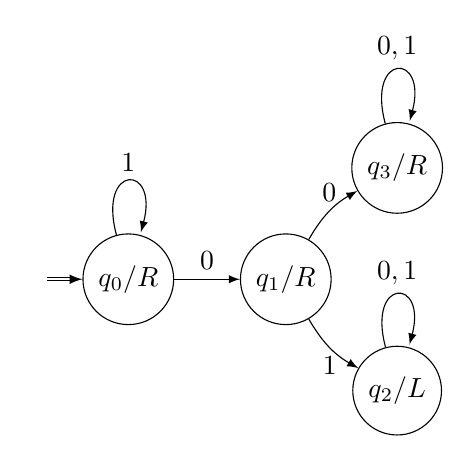
\begin{tikzpicture}[>=latex, node distance=2cm, initial text=, bend angle=15]
	\tikzstyle{every initial by arrow} = [->, double];

	\node [state, initial] (q_0)                        {$q_0/R$};
	\node [state]                     (q_1) [right of = q_0]  {$q_1/R$};
	\node [state]                     (q_2) [below right of = q_1] {$q_2/L$};
	\node [state]                     (q_3) [above right of = q_1] {$q_3/R$};

	\path [->] (q_0) edge [right] node [above]              {$0$}                 (q_1)
         		         edge [loop above] node [above]             {$1$}               ()
         			   (q_1) edge [bend left] node [above]             {$0$}                 (q_3)
         		         edge [bend right] node [below]             {$1$}              (q_2)
         			   (q_2)  edge [loop above] node [above]             {$0,1$}               ()
         			   (q_3)  edge [loop above] node [above]             {$0,1$}               ();
\end{tikzpicture}}
\end{minipage}
\begin{minipage}{0.05\linewidth}
\ \\
\end{minipage}
\begin{minipage}{0.5\linewidth}
\centering
\scalebox{0.035}{
\begin{tikzpicture}
  \draw[blue!50!black,rotate=270,l-system={rule set={X->X-YF,Y->FX+Y},
  step=100pt,angle=90,axiom=FX,order=10},-triangle 90] l-system;
\end{tikzpicture}}
\end{minipage}
\caption{
%Heighway dragon. 
(Left) A DFAO to output the direction (L/R) of $i$-th turn of the Heighway dragon given $i \ge 0$ in binary from the LSB as input. 
(Right) The first $2^{10}{-}1$ turns of the dragon. 
}
\label{fig:heighway_dragon}
\end{figure}

We shall initiate theoretical study on algorithmic self-assembly of shapes by cotranscriptional folding using oritatami system. 
Algorithmic cotranscriptional folding of Sierpinski triangle would allow us to borrow rich insights from the DNA tile self-assembly. 
On the other hand, in order to cut directly to the heart of algorithmic self-assembly by cotranscriptional folding, shapes of choice should be traversable by a sequence somehow algorithmically. 
One such way is to feed a turtle program (see \cite{AbelsondiSessa1981}) with an \textit{automatic sequence} as commands (drawing a line segment, rotation, etc.), whose $i$-th bit can be obtained by giving $i$ in binary from the least significant bit (LSB) to one deterministic finite automaton with output (DFAO) \cite{AlloucheShallit2003}.
%which can be generated by a deterministic finite automaton with output (DFAO) \cite{AlloucheShallit2003}. 
Shapes thus describable include the Heighway dragon \cite{AlloucheShallit2003} and von Koch curve \cite{MaHoldener2005}. 
A DFAO for the Heighway dragon is shown in Fig.~\ref{fig:heighway_dragon} (Left) and its output is as follows: 
%It is to read the binary representation of $i \ge 0$ from the LSB and outputs the $i$-th direction $P[i]$ to turn (L or R) assigned to the state finally reached as follows: 
\[
%\begin{array}{cccrrrrc}
%i 	&=& 0 &  2 & 6 & 14 & 30 & \cdots \\
%P[i] 	&=& {\rm R} & {\rm RL} & {\rm RRLL} & {\rm RRRLLRLL} & {\rm RRRLRRLLLRRLLRLL} & \cdots.
%\end{array}
P 	= {\rm RRLRRLLRRRLLRLLRRRLRRLLLRRLLRLL} \cdots.
\]
For instance, $i = 2$ is given in binary from the LSB as 01, with which the DFAO transitions as $q_0 \to q_1 \to q_2$ and hence $P[2] = L$. 
(The notation $P$ is after its appellative \textit{paperfolding sequence} \cite{AlloucheShallit2003}.) 
%where only the values of $i$ at the end of the first five iterations are specified. 
A turtle should interpret an L (resp.~R) as ``move forward by unit distance and turn left (resp. right) 90 degrees.''
Any portion of the dragon can be represented by a factor of $P$; for instance, Fig.~\ref{fig:heighway_dragon} (Right) depicts the factor $P[0 .. 1022]$, i.e., the first $2^{10}-1$ turns of the dragon. 

%\begin{figure}[htb]
\begin{wrapfigure}{l}{0.6\linewidth}
\vspace*{-5mm}
\centering
\includegraphics[width=\linewidth]{pic/6bit_heighway.pdf}
\caption{The portion $P[0 .. 62]$ of the Heighway dragon folded by the proposed oritatami system.}
\label{fig:heighway6_oritatami}
\end{wrapfigure}
%\end{figure}

In this paper, we propose a generic design of oritatami system for the algorithmic cotranscriptional folding of an arbitrary finite portion of the Heighway dragon. 
Fig.~\ref{fig:heighway6_oritatami} shows the portion $P[0 .. 62]$ thus folded (the dragon is slanted, but this is because the oritatami system operates on the triangular grid). 
The transcript is a repetition of three modules: a catenation of binary counters, DFAO module, and turning module. 
The counter is a technical modification of the one proposed in \cite{GeMeScSe2016}. 
By being fed with carry exactly once, the catenation can increment the count $i$ exactly by 1 while folding into a line segment, colored in red in Fig.~\ref{fig:heighway6_oritatami}. 
%It folds into one zigzag and increments a given binary number by 1 if carried-in or just propagates the number otherwise. 
%Binary counters fold into zigzags, yielding a (red) line segment of the dragon. 
%The system feeds only the first counter with carry so that the line segment amounts to increment the current count $i$ by 1. 
At the end of the segment comes a DFAO module, which computes the turn direction $P[i]$ while propagating the count $i$ to the following turning module. 
A (green) L-shaped block is the turning module. 
It is a concatenation of three bit-string bifurcation submodules, each of which folds into a rhombus, bifurcates the count $i$ and the direction $P[i]$ leftward as well as rightward, and directs the growth of further folding according to $P[i]$. 
We shall implement the DFAO and turning modules and verify them. 
The generic design brings the following theorem (for terminologies used, see Sect.~\ref{sect:preliminaries}) . 

\begin{theorem}\label{thm:main}
	For any finite portion $P[i..j]$ of the Heighway dragon, there exists an integer $c$ and a deterministic cyclic oritatami system of delay 3 and arity 3 that weakly folds into the $c$-rhombus scaling of $P[i..j]$. 
\end{theorem}

A JavaScript program to execute this oritatami system is freely available at \url{{\tt https://wolves13.github.io}}. 


%-------------------------------------------------------------------------------------------
	\section{Preliminaries}
%-------------------------------------------------------------------------------------------

Let $\Sigma$ be a set of types of abstract molecules, or \textit{beads}, and $\Sigma^*$ be the set of finite sequences of beads. 
A bead of type $a \in \Sigma$ is called an $a$-bead. 
Let $w = b_1 b_2\cdots b_n \in \Sigma^*$ be a string of length $n$ for some integer $n$ and bead types $b_1, \ldots, b_n \in \Sigma$.
The \textit{length} of $w$ is denoted by $|w|$, that is, $|w| = n$. 
For two indices $i,j$ with $1\leq i \leq j \leq n$, we let $w[i..j]$ refer to the subsequence $b_i b_{i+1} \cdots b_{j-1} b_{j}$; if $i=j$, then we simplify $w[i..i]$ as $w[i]$.
For $k \ge 1$, $w[1..k]$ is called a \textit{prefix} of $w$. 

Oritatami systems fold their transcript, a sequence of beads, over the triangular grid as suggested in Fig.~\ref{fig:glider} cotranscriptionally based on hydrogen-bond-based interactions (\textit{h-interactions} for short) which the rule set of the system allow for between adjacent beads of particular types. 
Let $\mathbb{T} = (V, E)$ be the triangular grid graph. 
A directed path $P = p_1 p_2 \cdots p_n$ in $\mathbb{T}$ is a sequence of \textit{pairwise-distinct} points $p_1, p_2, \ldots, p_n \in V$ such that $\{p_i, p_{i+1}\} \in E$ for all $1 \leq i < n$.
Its $i$-th point is referred to as $P[i]$. 
A \textit{rule set} $\mathcal{H} \subseteq \Sigma \times \Sigma$ is a symmetric relation over the set of pairs of bead types, that is, for all bead types $a, b \in \Sigma$, $(a, b) \in \mathcal{H}$ implies $(b, a) \in \mathcal{H}$. 

A \textit{conformation} $C$ is a triple $(P, w, H)$ of a directed path $P$ in $\mathbb{T}$, $w \in \Sigma^*$ of the same length as $P$, and a set of h-interactions $H \subseteq \{\{i,j\} \mid 1 \leq i, i+2 \leq j, \{P[i], P[j]\} \in E\}$.
This is to be interpreted as the sequence $w$ being folded in such a manner that its $i$-th bead $w[i]$ is placed on the $i$-th point $P[i]$ along the path and there is an h-interaction between the $i$-th and $j$-th beads if and only if $(i, j) \in H$. 
The condition $i+2 \leq j$ represents the topological restriction that two consecutive beads along the path cannot form an h-interaction between them.
Let $\mathcal{H}$ be a rule set. 
An h-interaction $(i, j) \in H$ is \textit{valid with respect to $\mathcal{H}$}, or simply \textit{$\mathcal{H}$-valid}, if $(w[i], w[j]) \in \mathcal{H}$. 
This conformation is $\mathcal{H}$-valid if all of its h-interactions are $\mathcal{H}$-valid. 
For an integer $\alpha \ge 1$, this conformation is \textit{of arity $\alpha$} if the maximum number of h-interactions per bead is $\alpha$, that is, if for any $k \ge 1$, $|\{i \mid (i, k) \in H)\}| + |\{j \mid (k, j) \in H\}| \le \alpha$ and this inequality holds as an equation of some $k$. 
By $\mathcal{C}_{\le \alpha}$, we denote the set of all conformations of arity at most $\alpha$.

Oritatami systems grow conformations by elongating them under their own rule set. 
Given a rule set $\mathcal{H}$ and an $\mathcal{H}$-valid finite conformation $C_1 = (P, w, H)$, 
we say that another conformation $C_2$ is an \textit{elongation of} $C_1$ \textit{by a bead} $b \in \Sigma$, written as $C_1 \xrightarrow{\mathcal{H}}_b C_2$, if $C_2 = (Pp, wb, H \cup H')$ for some point $p$ not along the path $P$ and set of h-interactions $H' \subseteq \left\{ \{i, |w|+1\} \bigm| 1\leq i < |w|, \{P[i], p\} \in E, (w[i], b) \in \mathcal{H}\right\}$, which can be empty.
Note that $C_2$ is also $\mathcal{H}$-valid.
This operation is recursively extended to the elongation by a finite sequence of beads as: 
for any conformation $C$, $C \xrightarrow{\mathcal{H}}^*_\lambda C$; 
and for a finite sequence of beads $w \in \Sigma^*$ and a bead $b \in \Sigma$,
a conformation $C_1$ is elongated to a conformation $C_2$ by the sequence $wb$,
written as $C_1 \xrightarrow{\mathcal{H}}^*_{wb} C_2$, if there is a conformation $C'$ that satisfies
$C_1 \xrightarrow{\mathcal{H}}^*_w C'$ and $C' \xrightarrow{\mathcal{H}}_b C_2$.

A finite \textit{oritatami system} (OS) is a 5-tuple $\Xi = (\mathcal{H}, \alpha, \delta, \sigma,w)$, where 
$\mathcal{H}$ is a rule set,
$\alpha$ is an arity, 
$\delta \geq 1$ is a parameter called the \textit{delay}, 
$\sigma$ is an initial $\mathcal{H}$-valid conformation of arity $\alpha$ called the \textit{seed}, upon which its finite \textit{transcript} $w \in \Sigma^*$ is to be folded by stabilizing beads of $w$ one at a time so as to minimize energy collaboratively with the succeeding $\delta -1$ nascent beads. 
The energy of a conformation $C = (P, w, H)$, denoted by $\Delta G(C)$, is defined to be $-|H|;$ the more h-interactions a conformation has, the more stable it gets.
The set $\mathcal{F}(\Xi)$ of conformations \textit{foldable} by this system is recursively defined as: 
the seed $\sigma$ is in $\mathcal{F}(\Xi)$; and provided that an elongation $C_{i}$ of $\sigma$ by the prefix $w[1..i]$ be foldable (i.e., $C_0 = \sigma$), its further elongation $C_{i+1}$ by the next bead $w[i+1]$ is foldable if
\begin{equation}\label{eq:cotranscriptional_folding}
C_{i+1} \in \argmin_{
\substack{
C \in \mathcal{C}_{\le \alpha} s.t. \\
C_i \xrightarrow{\mathcal{H}}_{w[i+1]}C \\
}
}
\min \Big\{ \Delta G(C') \mid 
C \xrightarrow{\mathcal{H}}^*_{w[i+2...i+k]}C', k\le \delta, C' \in \mathcal{C}_{\le \alpha}
\Big\}.
\end{equation}
We say that the bead $w[i+1]$ and the h-interactions it forms are \textit{stabilized} according to $C_{i+1}$.
Note that an arity-$\alpha$ OS cannot fold any conformation of arity larger than $\alpha$.
A conformation foldable by $\Xi$ is \textit{terminal} if none of its elongations is foldable by $\Xi$.

The OS $\Xi$ is \textit{deterministic} if for all $i \ge 0$, there exists at most one $C_{i+1}$ that satisfies \eqref{eq:cotranscriptional_folding}. 
Thus, a deterministic system folds into a unique terminal conformation. 
Let us provide an example of deterministic OS that folds into a motif of great use called the \textit{glider}. 

\begin{figure}[htb]
\centering
\scalebox{0.65}{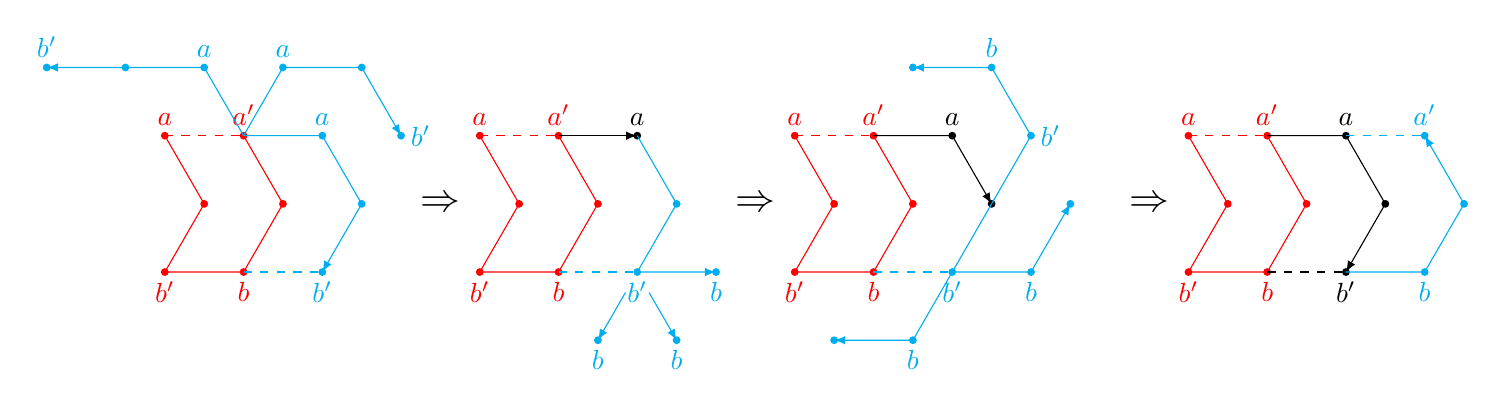
\begin{tikzpicture}
\tikzstyle{mol} = [fill,circle,inner sep=1pt]

\foreach \x in {0, 4, 8, 13} {
\draw[red] (\x, 0) node[mol] {} node[above] {$a$}
-- ++(300:1) node[mol] {} 
-- ++(240:1) node[mol] {} node[below] {$b'$}
-- ++(0:1) node[mol] {} node[below] {$b$}
-- ++(60:1) node[mol] {} 
-- ++(120:1) node[mol] {} node[above] {$a'$}
;
\draw[dashed,red] (\x, 0) -- ++(0:1);
}

\draw[cyan, -latex] (1, 0) -- ++(120:1) node[mol] {} node[above] {$a$} -- ++(180:1) node[mol]{} -- ++(180:1) node[mol] {} node[above] {$b'$};
\draw[cyan, -latex] (1, 0) -- ++(60:1) node[mol] {} node[above] {$a$} -- ++(0:1) node[mol] {} -- ++(300:1) node[mol] {} node[right] {$b'$};
\draw[cyan, -latex] (1, 0) -- ++(0:1) node[mol] {} node[above] {$a$} -- ++(300:1) node[mol] {} -- ++(240:1) node[mol] {} node[below] {$b'$};

\draw[dashed, cyan] (0,0)++(300:2) -- ++(0:1);

\draw (3,0)++(300:1) node {\Large $\Rightarrow$};
\draw (7,0)++(300:1) node {\Large $\Rightarrow$};
\draw (12,0)++(300:1) node {\Large $\Rightarrow$};


\draw[-latex] (5, 0) -- ++(0:1) node[mol] {} node[above] {$a$};

\draw[cyan, -latex] (6, 0) -- ++(300:1) node[mol] {} -- ++(240:1) node[mol] {} node[below] {$b'$} -- ++(0:1) node[mol] {} node[below] {$b$};
\draw[cyan, -latex] (5,0)++(300:2)++(240:0.3) -- ++(240:0.7) node[mol] {} node[below] {$b$};
\draw[cyan, -latex] (5,0)++(300:2.3) -- ++(300:0.7) node[mol] {} node[below] {$b$};
\draw[dashed, cyan] (4,0)++(300:2) -- ++(0:1);


\draw[-latex] (9, 0) -- ++(0:1) node[mol] {} node[above] {$a$}
-- ++(300:1) node[mol] {}
;
\draw[cyan, -latex] (10,0)++(300:1) -- ++(240:1) node[mol] {} node[below] {$b'$}
-- ++(240:1) node[mol] {} node[below] {$b$}
-- ++(180:1) node[mol] {}
;
\draw[cyan, -latex] (9,0)++(300:2) -- ++(0:1) node[mol] {} node[below] {$b$} -- ++(60:1) node[mol] {};
\draw[cyan, -latex] (10,0)++(300:1) -- ++(60:1) node[mol] {} node[right] {$b'$}
-- ++(120:1) node[mol] {} node[above] {$b$}
-- ++(180:1) node[mol] {}
;
\draw[cyan,dashed] (8,0)++(300:2) -- ++(0:1);

\draw[-latex] (14, 0) -- ++(0:1) node[mol] {} node[above] {$a$}
-- ++(300:1) node[mol] {}
-- ++(240:1) node[mol] {} node[below] {$b'$}
;
\draw[dashed] (13,0)++(300:2) -- ++(0:1);
\draw[cyan, -latex] (14,0)++(300:2) -- ++(0:1) node[mol] {} node[below] {$b$}
-- ++(60:1) node[mol] {}
-- ++(120:1) node[mol] {} node[above] {$a'$}
;
\draw[cyan,dashed] (15,0) -- ++(0:1);

\end{tikzpicture}}
\caption{Progression of a glider by distance 1.}
\label{fig:glider}
\end{figure}


\begin{example}\label{ex:glider}
%A motif called the \emph{glider} explains well how oritatami systems behave. 
Let $\Sigma = \{a, a', b, b', \bullet\}$. 
Consider a delay-3 oritatami system whose seed is colored in red in Figure~\ref{fig:glider} (left), transcript is a repetition of $a \bullet b' b \bullet a'$, and the rule set is $\mathcal{H} = \{(a, a'), (b, b')\}$, which makes $\bullet$-beads inert. 

By the fragment $a \bullet b'$ of the first three beads of the transcript, the seed can be elongated in many ways; three of them are shown in Figure~\ref{fig:glider} (left). 
The only bead on the fragment capable of a new h-interaction is $b'$ (with a $b$-bead).
In order for the $b'$-bead to form an h-interaction with a $b$-bead, the first $a$-bead must be located to the east of the last bead of the seed. 
Thus, the $a$-bead is stabilized there. 
The next bead is then transcribed, which is of type $b$.
It is not capable of any h-interaction because any $b'$ around is either too far or too close.  
Hence, the nascent fragment $\bullet b' b$ gets stabilized as being folded as done before up to at least the first two beads. 
The $\bullet$ bead is stabilized southeastward. 
%Thus, the only way for the nascent fragment $\bullet b' b$ to form an h-interaction is to let the $b'$ bind as done before, and for that, the $\bullet$ must be located to the southeast of the preceding $a$. 
An inert bead pops up next so that the $b'$ gets stabilized southwestward as suggested before. 
The first three beads $a, \bullet, b'$ have been thus stabilized and the glider has moved forward by unit distance. 
It is easily induced inductively that gliders of arbitrary ``flight distance'' can be folded. 


Gliders also provide a medium to propagate 1-bit straight at arbitrary distance. 
The height (top or bottom) of the first bead determines whether the last bead is stabilized top or bottom after flying a given distance.
For instance, the glider in Figure~\ref{fig:glider} launches top and thus its last bead (the $a'$) also comes top after traveling the distance 2.
The oritatami system we shall propose exploits this information-carrying capability.
\end{example}


%-------------------------------------------------------------------------------------------
	\section{Heighway dragon oritatami system}
%-------------------------------------------------------------------------------------------

We propose a generic design of deterministic oritatami system that allows us to fold an arbitrary finite portion of the Heighway dragon. 
The design concept has been already explained in the introduction. 
The dragon it folds into is actually slanted as illustrated in Figure~\ref{fig:heighway6_oritatami}, which is more natural than the conventional (upright) one to be folded over the triangular grid. 
The design sets both delay and arity to 3 and employs a fixed number of bead types (about 2000), no matter which portion is folded. 
Minimizing the number of bead types has just proven NP-hard \cite{HanKim2017}. 

Any finite portion of the Heighway dragon is expected to be foldable by \textit{hard-coding} if an arbitrary number of bead types is available and the shape can be scaled-up (though, if rescaling is not allowed, it is NP-hard to decide if for a given finite shape, there exists an oritatami system that folds into the shape \cite{PatitzRogers2017}). 
The proposed design cannot take this approach because the number of bead types available is fixed. 
An oritatami system $\Xi = (\mathcal{H}, \alpha, \delta, \sigma, w)$ that the design provides is periodic in the sense that its transcript is a periodic sequence. 
If this system is for the $n$-th repetition of the Heighway dragon, then the length of its period is $|w|/2^{n-1}$. 
One period corresponds to a successive two pairs of a red line segment and the following green L-shaped block. 

Why do these two pairs have to be distinguished from each other? 
The answer to this question lies in the fact that the Heighway dragon is slanted. 
The slanted dragon involves two types of left turn as well as two types of right turn: acute and obtuse. 
Capability of one turning module to make all of the four possible turns would shorten the period by half. 
Such a turning module, however, would have to take quite a large number of conformations; recall that what the module has to turn is not a straw but a thick wire which bears the current count $i$. 
Implementing such a module totally ignores the level of oritatami design techniques accumulated so far.  
Our approach makes it sufficient to implement a turning module capable of just an acute turn and an obtuse turn. 
Observe that after the (slanted) vertical segment, certainly the left turn is obtuse while the right turn is acute, whereas after the horizontal segment, the left turn is acute while the right turn is obtuse. 
In addition, we know \textit{a priori} which segments are vertical and which are horizontal; indeed vertical segments and horizontal segments occur alternately on the Heighway dragon. 
Therefore, we can attach a proper interpreter to a DFAO module to convert its output L/R into a signal A(cute)/O(btuse). 
Two types of interpreters are hence needed: vertical interpreter converts L into obtuse and R into acute, while horizontal one converts them the other way around. 

\begin{figure}[h]
\includegraphics[width=\linewidth]{pic/dragon_vol4.pdf}
\caption{
Folding of one segment plus turn of the Heighway dragon, flow of information through it, and two ways of collision avoidance between two turns.
}
\label{fig:abst_dragon}
\end{figure}

The sole difference between the first and second halves of a period is anyway the type of interpreter (AO or $\overline{\rm AO}$). 
Thus, it should be sufficient to explain only the first half. 
The half consists of four subsequences for the counter, copier, DFAO, and turning modules. 
It folds as abstracted in Figure~\ref{fig:abst_dragon} into one line segment plus one turn of the Heighway dragon and has its four modules accomplish the following processes, respectively: 
\begin{enumerate}[itemsep=0pt]
\item $i \gets i + 1$ (count-up)
\item Copy $i$ (drawing a line segment)
\item Compute $P[i]$
\item Make a turn according to $P[i]$
\end{enumerate}
Its length is proportional to $n^2$ and hence so is the length of a period. 
The seed of the system replaces the counter module at the beginning of the first period and encodes the initial value of $i$ as a sequence of bead types in an appropriate format such that copier modules can ``read'' the count $i$. 
We shall explain how modules read something in Section~\ref{subsubsec:module_counter}. 
Before explaining the implementation of each module, we should point out one significant issue specific to the folding by oritatami systems. 
It rises when the Heighway dragon makes a turn where it has already made another turn before, that is, when two turns share a point. 
By definition, oritatami systems cannot put a bead anywhere occupied by another bead. 
This is the reason of the L-shape of the turning module. 
As shown in Figures~\ref{fig:heighway6_oritatami} and \ref{fig:abst_dragon}, the proposed system makes an acute turn by having three bifurcation components direct the growth of further folding acutely one after another, while an obtuse turn by having them direct the growth rather obtusely. 

%-------------------------------------------------------------------------------------------
		\subsection{Modules}
%-------------------------------------------------------------------------------------------

Now it suffices to explain how modules and their components are implemented, interlocked with each other, and collaborate. 
Using the simulator developed for \cite{HaKiOtSe2016}, we have verified that all of the components fold correctly in all possible environments, which are abstracted in Figures~\ref{fig:abst_dragon}, \ref{fig:abst_dfao}, and \ref{fig:overall_turning}. 

%-------------------------------------------------------------------------------------------
			\subsubsection{Counter and copier modules}
			\label{subsubsec:module_counter}
%-------------------------------------------------------------------------------------------

The existing binary counter \cite{GeMeScSe2016} was modified so as to operate in the dynamics \eqref{eq:cotranscriptional_folding}, which is more prevailing \cite{GeMeScSe2015,HanKim2017,HaKiOtSe2016,OtaSeki2017} but less tractable than the one the original counter used. 

%%%%%%%%%%%%%%%%%%%%%%%%%%%%%%%%%%%%%%%%%%%%
\begin{figure}[h]
\begin{tabular}{c}

%%%%%%%%%%%%Counter-zig-01%%%%%%%%%%%%%%%%%
\begin{minipage}{0.25\hsize}
\centering
\scalebox{0.8}{
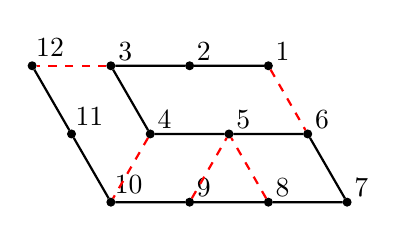
\begin{tikzpicture}[node distance=1cm,every node/.style={draw,circle,fill,inner sep=1pt}]
   \node (7) at (0:0)[label=above right:7]{};
  \node (6) at (120:1)[label=above right:6]{};
  \node (1)at (120:2)[label=above right:1]{};
  \node[left of= 7] (8) [label=above right:8]{};
  \node[left of =8](9)[label=above right:9]{};
  \node[left of =9](10)[label=above right:10]{};
  \node[left of =6](5)[label=above right:5]{};
  \node[left of =5](4)[label=above right:4]{};
  \node[left of =4](11)[label=above right:11]{};
  \node[left of =1](2)[label=above right:2]{};
  \node[left of =2](3)[label=above right:3]{};
  \node[left of =3](12)[label=above right:12]{};
  \draw[thick](1)--(2)--(3)--(4)--(5)--(6)--(7)--(8)--(9)--(10)--(11)--(12);
  \draw[dashed,thick,red](1)--(6);
  \draw[dashed,thick,red](4)--(10);
 \draw[dashed,thick,red](9)--(5);
\draw[dashed,thick,red](8)--(5);
\draw[dashed,thick,red](3)--(12);
  \end{tikzpicture}
  }
\end{minipage}

%%%%%%%%%%%%Counter-zig-10%%%%%%%%%%%%%%%%%
\begin{minipage}{0.25\hsize}
\centering
\scalebox{0.8}{
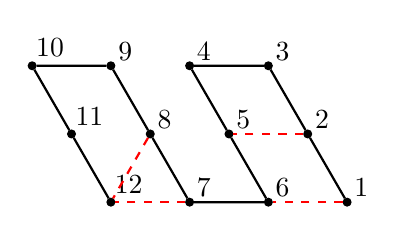
\begin{tikzpicture}[node distance=1cm,every node/.style={draw,circle,fill,inner sep=1pt}]
   \node (1) at (0:0)[label=above right:1]{};
  \node (2) at (120:1)[label=above right:2]{};
  \node (3)at (120:2)[label=above right:3]{};
  \node[left of= 1] (6) [label=above right:6]{};
  \node[left of =6](7)[label=above right:7]{};
  \node[left of =7](12)[label=above right:12]{};
  \node[left of =2](5)[label=above right:5]{};
  \node[left of =5](8)[label=above right:8]{};
  \node[left of =8](11)[label=above right:11]{};
  \node[left of =3](4)[label=above right:4]{};
  \node[left of =4](9)[label=above right:9]{};
  \node[left of =9](10)[label=above right:10]{};
  \draw[thick](1)--(2)--(3)--(4)--(5)--(6)--(7)--(8)--(9)--(10)--(11)--(12);
  \draw[dashed,thick,red](1)--(6);
\draw[dashed,thick,red](2)--(5);
\draw[dashed,thick,red](8)--(12);
\draw[dashed,thick,red](7)--(12);
  \end{tikzpicture}
}
\end{minipage}

%%%%%%%%%%%%Counter-zig-00%%%%%%%%%%%%%%%%%
\begin{minipage}{0.25\hsize}
\centering
\scalebox{0.8}{
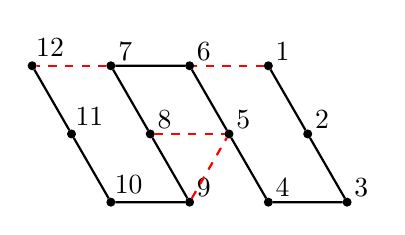
\begin{tikzpicture}[node distance=1cm,every node/.style={draw,circle,fill,inner sep=1pt}]
   \node (3) at (0:0)[label=above right:3]{};
  \node (2) at (120:1)[label=above right:2]{};
  \node (1)at (120:2)[label=above right:1]{};
  \node[left of= 3] (4) [label=above right:4]{};
  \node[left of =4](9)[label=above right:9]{};
  \node[left of =9](10)[label=above right:10]{};
  \node[left of =2](5)[label=above right:5]{};
  \node[left of =5](8)[label=above right:8]{};
  \node[left of =8](11)[label=above right:11]{};
  \node[left of =1](6)[label=above right:6]{};
  \node[left of =6](7)[label=above right:7]{};
  \node[left of =7](12)[label=above right:12]{};
  \draw[thick](1)--(2)--(3)--(4)--(5)--(6)--(7)--(8)--(9)--(10)--(11)--(12);
  \draw[dashed,thick,red](1)--(6);
  \draw[dashed,thick,red](7)--(12);
 \draw[dashed,thick,red](9)--(5);
\draw[dashed,thick,red](8)--(5);
\end{tikzpicture}
}
\end{minipage}


%%%%%%%%%%%%Counter-zig-11%%%%%%%%%%%%%%%%%
\begin{minipage}{0.25\hsize}
\centering
\scalebox{0.8}{
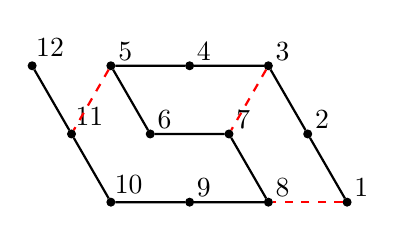
\begin{tikzpicture}[node distance=1cm,every node/.style={draw,circle,fill,inner sep=1pt}]
   \node (1) at (0:0)[label=above right:1]{};
  \node (2) at (120:1)[label=above right:2]{};
  \node (3)at (120:2)[label=above right:3]{};
  \node[left of= 1] (8) [label=above right:8]{};
  \node[left of =8](9)[label=above right:9]{};
  \node[left of =9](10)[label=above right:10]{};
  \node[left of =2](7)[label=above right:7]{};
  \node[left of =7](6)[label=above right:6]{};
  \node[left of =6](11)[label=above right:11]{};
  \node[left of =3](4)[label=above right:4]{};
  \node[left of =4](5)[label=above right:5]{};
  \node[left of =5](12)[label=above right:12]{};
  \draw[thick](1)--(2)--(3)--(4)--(5)--(6)--(7)--(8)--(9)--(10)--(11)--(12);
  \draw[dashed,thick,red](1)--(8);
\draw[dashed,thick,red](3)--(7);
\draw[dashed,thick,red](5)--(11);
  \end{tikzpicture}
}
\end{minipage}

\end{tabular}
 \caption{All conformations of the half-adder component.}
\label{fig:half-adder}
\end{figure}
%%%%%%%%%%%%%%%%%%%%%%%%%%%%%%%%%%%%%%%%%%%%

The essential component of this module is the half-adder. 
In Figure~\ref{fig:abst_dragon}, half-adder components are abstracted as small rhombuses at the top labeled with $a_n, a_{n-1}, \ldots, a_1$, where the one with $a_j$ is for the $j$-th bit of the current count $i$. 
Though not described, two horizontally adjacent half-adders sandwitch a glider of even length as a space to keep them away from each other sufficiently to prevent any undesirable interference. 
Figure~\ref{fig:half-adder} illustrates its four possible conformations. 
The whole oritatami system is designed in such a manner that a 1-bit input (1 or 0) is exposed to the specific position (colored red or yellow in Figure~\ref{fig:half-adder}) as a pair of bead types by the previous turning module. 
The system is also designed in such a manner that a half-adder starts folding either at the top, as in the first and third conformations, or at the bottom as in the other two. 
The half-adder considers the top start position as non-carry and the bottom start position as carry. 
Thus, only when a half-adder takes 1 and carry, it ends at the bottom (second conformation in Figure~\ref{fig:half-adder}), which is propagated to the next half-adder as it is via the spacer between them. 
These four conformations expose sequences of four bead types below that are distinct enough to convey the intended 1-bit output to another computing component, or in other words, we can design a component that can ``read'' the output. 
From this point forward, conformations for other components will be illustrated; their input and output will be labeled by their meaning mutually understood by the components that exchange them. 

Being fed with non-carry, the counter module serves as the copier module. 
Combining them one after another yields a line segment of arbitrary length, through which the current count $i$ is propagated. 


%-------------------------------------------------------------------------------------------
			\subsubsection{DFAO module}
%-------------------------------------------------------------------------------------------


A DFAO module receives the current count $i$ from the last copier module, computes $P[i]$, interprets it properly either A or O, and outputs it together with the count $i$ at the very end of a red line segment. 

\begin{figure}[h]
\includegraphics[width=\linewidth]{pic/abst_DFAO.pdf}
\caption{Component-level abstraction of the folding of DFAO module.}
\label{fig:abst_dfao}
\end{figure}

%%%%%%%%%%%%%%%%%%%%%%%%%%%%%%%%%%%%%%%%%%%%

\begin{figure}[h]
\begin{tabular}{c}

%%%%%%%%%%%%PFS-L%%%%%%%%%%%%%%%%%
\begin{minipage}{0.2\hsize}
\centering
\scalebox{0.75}{
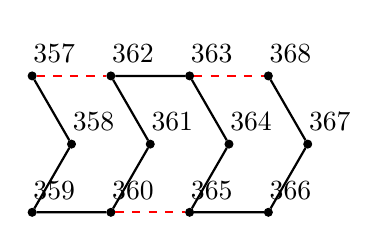
\begin{tikzpicture}[node distance=1cm,every node/.style={draw,circle,fill,inner sep=1pt}]
  \node (3) at (0:0)[label=above right:359]{};
  \node (2) at (60:1)[label=above right:358]{};
  \node (6)at (60:2)[label=above right:362]{};
  \node[right of =3](4)[label=above right:360]{};
  \node[right of =4](9)[label=above right:365]{};
  \node[right of =9](10)[label=above right:366]{};
  \node[right of =2](5)[label=above right:361]{};
  \node[right of =5](8)[label=above right:364]{};
  \node[right of =8](11)[label=above right:367]{};
  \node[left of= 6] (1) [label=above right:357]{};
  \node[right of =6](7)[label=above right:363]{};
  \node[right of =7](12)[label=above right:368]{};
  \draw[thick](1)--(2)--(3)--(4)--(5)--(6)--(7)--(8)--(9)--(10)--(11)--(12);
  \draw[dashed,thick,red](1)--(6);
  \draw[dashed,thick,red](4)--(9);
  \draw[dashed,thick,red](7)--(12);
  \end{tikzpicture}
}
\end{minipage}

\begin{minipage}{0.03\hsize}
\ \\
\end{minipage}

%%%%%%%%%%%%PFS-R%%%%%%%%%%%%%%%%%
\begin{minipage}{0.2\hsize}
\centering
\scalebox{0.75}{
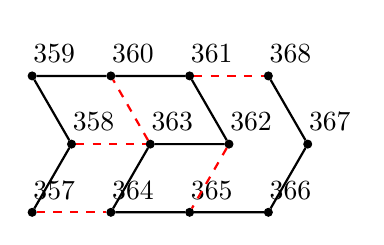
\begin{tikzpicture}[node distance=1cm,every node/.style={draw,circle,fill,inner sep=1pt}]
  \node (1) at (0:0)[label=above right:357]{};
  \node (2) at (60:1)[label=above right:358]{};
  \node (4)at (60:2)[label=above right:360]{};
  \node[right of =1](8)[label=above right:364]{};
  \node[right of =8](9)[label=above right:365]{};
  \node[right of =9](10)[label=above right:366]{};
  \node[right of =2](7)[label=above right:363]{};
  \node[right of =7](6)[label=above right:362]{};
  \node[right of =6](11)[label=above right:367]{};
  \node[left of= 4] (3) [label=above right:359]{};
  \node[right of =4](5)[label=above right:361]{};
  \node[right of =5](12)[label=above right:368]{};
  \draw[thick](1)--(2)--(3)--(4)--(5)--(6)--(7)--(8)--(9)--(10)--(11)--(12);
  \draw[dashed,thick,red](1)--(8);
  \draw[dashed,thick,red](2)--(7);
  \draw[dashed,thick,red](7)--(4);
  \draw[dashed,thick,red](6)--(9);
  \draw[dashed,thick,red](5)--(12);
  \end{tikzpicture}
}

\end{minipage}

\begin{minipage}{0.04\hsize}
\ \\
\end{minipage}

%%%%%%%%%%%%AO-A%%%%%%%%%%%%%%%%%
\begin{minipage}{0.2\hsize}
\scalebox{0.75}{
  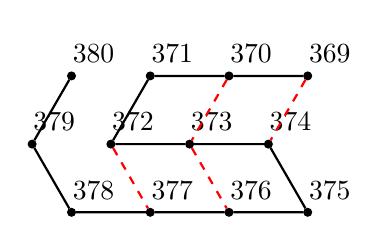
\begin{tikzpicture}[node distance=1cm,every node/.style={draw,circle,fill,inner sep=1pt}]
  \node (7) at (0:0)[label=above right:375]{};
  \node (6) at (120:1)[label=above right:374]{};
  \node (2) at (120:2)[label=above right:370]{};
  \node[left of =7](8)[label=above right:376]{};
  \node[left of =8](9)[label=above right:377]{};
  \node[left of =9](10)[label=above right:378]{};
  
  \node[left of =6](5)[label=above right:373]{};
  \node[left of =5](4)[label=above right:372]{};
  \node[left of =4](11)[label=above right:379]{};
  
  \node[right of= 2](1)[label=above right:369]{};

  \node[left of =2](3)[label=above right:371]{};
  \node[left of =3](12)[label=above right:380]{};
  \draw[thick](1)--(2)--(3)--(4)--(5)--(6)--(7)--(8)--(9)--(10)--(11)--(12);
  \draw[dashed,thick,red](1)--(6);
  \draw[dashed,thick,red](2)--(5);
  \draw[dashed,thick,red](5)--(8);
  \draw[dashed,thick,red](4)--(9);
  
  \end{tikzpicture}
  }
\end{minipage}  

\begin{minipage}{0.03\hsize}
\ \\
\end{minipage}

%%%%%%%%%%%%AO-O%%%%%%%%%%%%%%%%%
\begin{minipage}{0.2\hsize}
\scalebox{0.75}{
  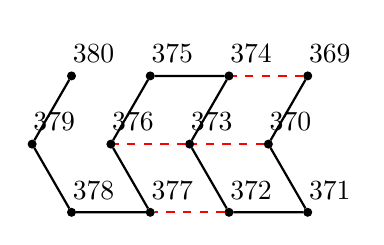
\begin{tikzpicture}[node distance=1cm,every node/.style={draw,circle,fill,inner sep=1pt}]
  \node (3) at (0:0)[label=above right:371]{};
  \node (2) at (120:1)[label=above right:370]{};
  \node (6)at (120:2)[label=above right:374]{};


  \node[left of =3](4)[label=above right:372]{};
  \node[left of =4](9)[label=above right:377]{};
  \node[left of =9](10)[label=above right:378]{};
  
  \node[left of =2](5)[label=above right:373]{};
  \node[left of =5](8)[label=above right:376]{};
  \node[left of =8](11)[label=above right:379]{};
  
  \node[right of= 6](1)[label=above right:369]{};
  \node[left of =6](7)[label=above right:375]{};
  \node[left of =7](12)[label=above right:380]{};
  \draw[thick](1)--(2)--(3)--(4)--(5)--(6)--(7)--(8)--(9)--(10)--(11)--(12);
  \draw[dashed,thick,red](1)--(6);
  \draw[dashed,thick,red](2)--(5);
  \draw[dashed,thick,red](5)--(8);
  \draw[dashed,thick,red](4)--(9);
  \end{tikzpicture}
  }
\end{minipage}  

\end{tabular}
\caption{(left) The possible two conformations of PFS: PFS-L, PFS-R. (right) The possible two conformations of AO.}
\label{fig:PFS}
\end{figure}
%%%%%%%%%%%%%%%%%%%%%%%%%%%%%%%%%%%%%%%%%%%%


DFAO is composed of the six components: DFAO-zig, DFAO-zag1, DFAO-zig2, DFAO-zag2, PFS, AO (or  ``$\overline{\rm AO}$").
At the component-level, it folds into two zig-zags as abstracted in Figure~\ref{fig:abst_dfao}.
What the module does in the first zig-zag is to have DFAO-zig1s and DFAO-zag1s read the current count $i$ from its LSB and ``mark" the first 0, while propagating $i$.
In the second zig-zag, it employs DFAO-zig2s and DFAO-zag2s to check whether the automaton transitions to the state $q_2$ ($P_i = L$) or else ($P_i = R$).
The second zag is to end at the top if $P_i = L$ or at the bottom if $P_i = R$.
PFS takes one of the two conformations in Fig.~\ref{fig:PFS} and outputs $P_i$ downward.
In vertical segments, PFS is followed by AO, while in horizontal segments, it is followed by $\overline{\rm AO}$.
AO interprets the PFS' output $P_i = R$ as acute and $P_i = L$ as obtuse, as shown in Fig.~\ref{fig:PFS}.
$\overline{\rm AO}$ interprets them the other way around.
Let us explain briefly how each of the components folds to fulfill its roles.

%%%%%%%%%%%%%%%%%%%%%%%%%%%%%%%%%%%%%%%%%%%%
\begin{figure}[h]
\begin{tabular}{c}
%%%%%%%%%%%%Dzig1-1%%%%%%%%%%%%%%%%%
\begin{minipage}{0.4\hsize}
\centering
\scalebox{0.75}{
  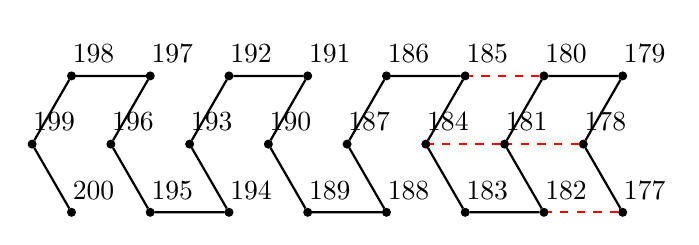
\begin{tikzpicture}[node distance=1cm,every node/.style={draw,circle,fill,inner sep=1pt}]
  \node (1) at (0:0)[label=above right:177]{};
  \node (2) at (120:1)[label=above right:178]{};
  \node (4)at (120:2)[label=above right:180]{};


  \node[right of =4](3)[label=above right:179]{};
  \node[left of =4](9)[label=above right:185]{};
  \node[left of =9](10)[label=above right:186]{};
  \node[left of =10](15)[label=above right:191]{};
  \node[left of =15](16)[label=above right:192]{};
  \node[left of =16](21)[label=above right:197]{};
  \node[left of =21](22)[label=above right:198]{};
  
  \node[left of =2](5)[label=above right:181]{};
  \node[left of =5](8)[label=above right:184]{};
  \node[left of =8](11)[label=above right:187]{};
  \node[left of =11](14)[label=above right:190]{};
  \node[left of =14](17)[label=above right:193]{};
  \node[left of =17](20)[label=above right:196]{};
  \node[left of =20](23)[label=above right:199]{};
  
  \node[left of= 1](6)[label=above right:182]{};
  \node[left of =6](7)[label=above right:183]{};
  \node[left of =7](12)[label=above right:188]{};
  \node[left of =12](13)[label=above right:189]{};
  \node[left of =13](18)[label=above right:194]{};
  \node[left of =18](19)[label=above right:195]{};
  \node[left of =19](24)[label=above right:200]{};
  
  \draw[thick](1)--(2)--(3)--(4)--(5)--(6)--(7)--(8)--(9)--(10)--(11)--(12)--(13)--(14)--(15)--(16)--(17)--(18)--(19)--(20)--(21)--(22)--(23)--(24);
  \draw[dashed,thick,red](1)--(6);
  \draw[dashed,thick,red](2)--(5);
  \draw[dashed,thick,red](5)--(8);
  \draw[dashed,thick,red](4)--(9);
  \end{tikzpicture}
  }
\end{minipage}

\begin{minipage}{0.1\hsize}
\ \\
\end{minipage}

%%%%%%%%%%%%Dzig1-f0%%%%%%%%%%%%%%%%%
\begin{minipage}{0.4\hsize}
\centering
\scalebox{0.75}{
   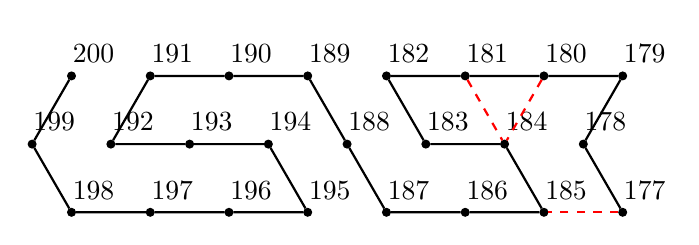
\begin{tikzpicture}[node distance=1cm,every node/.style={draw,circle,fill,inner sep=1pt}]
  \node (1) at (0:0)[label=above right:177]{};
  \node (2) at (120:1)[label=above right:178]{};
  \node (4)at (120:2)[label=above right:180]{};


  \node[right of =4](3)[label=above right:179]{};
  \node[left of =4](5)[label=above right:181]{};
  \node[left of =5](6)[label=above right:182]{};
  \node[left of =6](13)[label=above right:189]{};
  \node[left of =13](14)[label=above right:190]{};
  \node[left of =14](15)[label=above right:191]{};
  \node[left of =15](24)[label=above right:200]{};
  
  \node[left of =2](8)[label=above right:184]{};
  \node[left of =8](7)[label=above right:183]{};
  \node[left of =7](12)[label=above right:188]{};
  \node[left of =12](18)[label=above right:194]{};
  \node[left of =18](17)[label=above right:193]{};
  \node[left of =17](16)[label=above right:192]{};
  \node[left of =16](23)[label=above right:199]{};
  
  \node[left of= 1](9)[label=above right:185]{};
  \node[left of =9](10)[label=above right:186]{};
  \node[left of =10](11)[label=above right:187]{};
  \node[left of =11](19)[label=above right:195]{};
  \node[left of =19](20)[label=above right:196]{};
  \node[left of =20](21)[label=above right:197]{};
  \node[left of =21](22)[label=above right:198]{};
  
  \draw[thick](1)--(2)--(3)--(4)--(5)--(6)--(7)--(8)--(9)--(10)--(11)--(12)--(13)--(14)--(15)--(16)--(17)--(18)--(19)--(20)--(21)--(22)--(23)--(24);
  \draw[dashed,thick,red](1)--(9);
  \draw[dashed,thick,red](5)--(8);
  \draw[dashed,thick,red](4)--(8);
  \end{tikzpicture}
  }
\end{minipage}

 \\
 \\
%%%%%%%%%%%%Dzig1-20%%%%%%%%%%%%%%%%%
\begin{minipage}{0.4\hsize}
\centering
\scalebox{0.75}{
  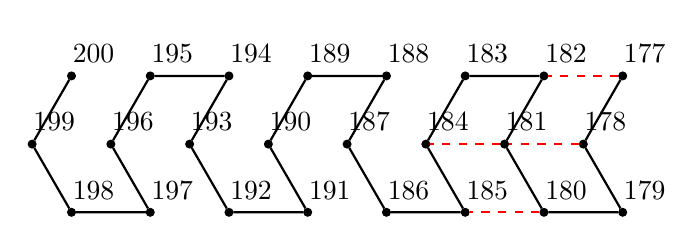
\begin{tikzpicture}[node distance=1cm,every node/.style={draw,circle,fill,inner sep=1pt}]
  \node (3) at (0:0)[label=above right:179]{};
  \node (2) at (120:1)[label=above right:178]{};
  \node (6)at (120:2)[label=above right:182]{};


  \node[left of =3](4)[label=above right:180]{};
  \node[left of =4](9)[label=above right:185]{};
  \node[left of =9](10)[label=above right:186]{};
  \node[left of =10](15)[label=above right:191]{};
  \node[left of =15](16)[label=above right:192]{};
  \node[left of =16](21)[label=above right:197]{};
  \node[left of =21](22)[label=above right:198]{};
  
  \node[left of =2](5)[label=above right:181]{};
  \node[left of =5](8)[label=above right:184]{};
  \node[left of =8](11)[label=above right:187]{};
  \node[left of =11](14)[label=above right:190]{};
  \node[left of =14](17)[label=above right:193]{};
  \node[left of =17](20)[label=above right:196]{};
  \node[left of =20](23)[label=above right:199]{};
  
  \node[right of= 6](1)[label=above right:177]{};
  \node[left of =6](7)[label=above right:183]{};
  \node[left of =7](12)[label=above right:188]{};
  \node[left of =12](13)[label=above right:189]{};
  \node[left of =13](18)[label=above right:194]{};
  \node[left of =18](19)[label=above right:195]{};
  \node[left of =19](24)[label=above right:200]{};
  
  \draw[thick](1)--(2)--(3)--(4)--(5)--(6)--(7)--(8)--(9)--(10)--(11)--(12)--(13)--(14)--(15)--(16)--(17)--(18)--(19)--(20)--(21)--(22)--(23)--(24);
  \draw[dashed,thick,red](1)--(6);
  \draw[dashed,thick,red](2)--(5);
  \draw[dashed,thick,red](5)--(8);
  \draw[dashed,thick,red](4)--(9);
  \end{tikzpicture}
  }
\end{minipage}

\begin{minipage}{0.1\hsize}
\ \\
\end{minipage}

%%%%%%%%%%%%Dzig1-21%%%%%%%%%%%%%%%%%
\begin{minipage}{0.4\hsize}
\centering
\scalebox{0.75}{
  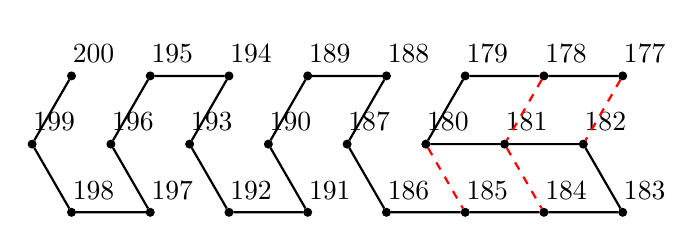
\begin{tikzpicture}[node distance=1cm,every node/.style={draw,circle,fill,inner sep=1pt}]
  \node (7) at (0:0)[label=above right:183]{};
  \node (6) at (120:1)[label=above right:182]{};
  \node (2)at (120:2)[label=above right:178]{};


  \node[left of =7](8)[label=above right:184]{};
  \node[left of =8](9)[label=above right:185]{};
  \node[left of =9](10)[label=above right:186]{};
  \node[left of =10](15)[label=above right:191]{};
  \node[left of =15](16)[label=above right:192]{};
  \node[left of =16](21)[label=above right:197]{};
  \node[left of =21](22)[label=above right:198]{};
  
  \node[left of =6](5)[label=above right:181]{};
  \node[left of =5](4)[label=above right:180]{};
  \node[left of =4](11)[label=above right:187]{};
  \node[left of =11](14)[label=above right:190]{};
  \node[left of =14](17)[label=above right:193]{};
  \node[left of =17](20)[label=above right:196]{};
  \node[left of =20](23)[label=above right:199]{};
  
  \node[right of= 2](1)[label=above right:177]{};
  \node[left of =2](3)[label=above right:179]{};
  \node[left of =3](12)[label=above right:188]{};
  \node[left of =12](13)[label=above right:189]{};
  \node[left of =13](18)[label=above right:194]{};
  \node[left of =18](19)[label=above right:195]{};
  \node[left of =19](24)[label=above right:200]{};
  
  \draw[thick](1)--(2)--(3)--(4)--(5)--(6)--(7)--(8)--(9)--(10)--(11)--(12)--(13)--(14)--(15)--(16)--(17)--(18)--(19)--(20)--(21)--(22)--(23)--(24);
  \draw[dashed,thick,red](1)--(6);
  \draw[dashed,thick,red](2)--(5);
  \draw[dashed,thick,red](5)--(8);
  \draw[dashed,thick,red](4)--(9);
  \end{tikzpicture}
  }
\end{minipage}
  
\end{tabular}
  \caption{The possible four conformations of DFAO-zig1: (top) Dzig1-1 and Dzig1-f0; (bottom) Dzig1-20 and Dzig1-21.}
  \label{fig:DFAO-zig1}
\end{figure} 

%%%%%%%%%%%%%%%%%%%%%%%%%%%%%%%%%%%%%%%%%%%%%%%%%%%%

\begin{figure}[h]
\begin{tabular}{c}

%%%%%%%%%%%%%%Dzag-f0%%%%%%%%%%%%%%%%%
\begin{minipage}{0.3\hsize}
\centering
\scalebox{0.5}{
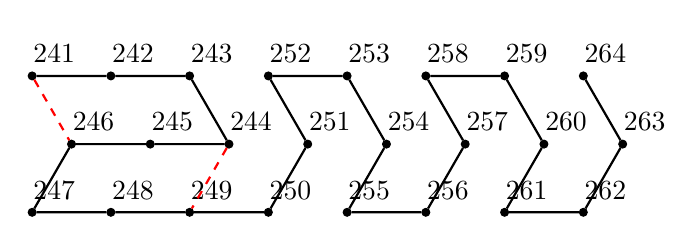
\begin{tikzpicture}[node distance=1cm,every node/.style={draw,circle,fill,inner sep=1pt}]
  \node (7) at (0:0)[label=above right:247]{};
  \node (6) at (60:1)[label=above right:246]{};
  \node (2)at (60:2)[label=above right:242]{};
  
  \node[right of =7](8)[label=above right:248]{};
  \node[right of =8](9)[label=above right:249]{};
  \node[right of =9](10)[label=above right:250]{};
  \node[right of =10](15)[label=above right:255]{};
  \node[right of =15](16)[label=above right:256]{};
  \node[right of =16](21)[label=above right:261]{};
  \node[right of =21](22)[label=above right:262]{};
  
  \node[right of =6](5)[label=above right:245]{};
  \node[right of =5](4)[label=above right:244]{};
  \node[right of =4](11)[label=above right:251]{};
  \node[right of =11](14)[label=above right:254]{};
  \node[right of =14](17)[label=above right:257]{};
  \node[right of =17](20)[label=above right:260]{};
  \node[right of =20](23)[label=above right:263]{};
  
  \node[left of= 2] (1) [label=above right:241]{};
  \node[right of =2](3)[label=above right:243]{};
  \node[right of =3](12)[label=above right:252]{};
  \node[right of =12](13)[label=above right:253]{};
  \node[right of =13](18)[label=above right:258]{};
  \node[right of =18](19)[label=above right:259]{};
  \node[right of =19](24)[label=above right:264]{};
  
  
  \draw[thick](1)--(2)--(3)--(4)--(5)--(6)--(7)--(8)--(9)--(10)--(11)--(12)--(13)--(14)--(15)--(16)--(17)--(18)--(19)--(20)--(21)--(22)--(23)--(24);
  \draw[dashed,thick,red](1)--(6);
  \draw[dashed,thick,red](4)--(9);
  \end{tikzpicture}
  }
  \end{minipage}
  
\begin{minipage}{0.05\hsize}
\ \\
\end{minipage}

%%%%%%%%%%%%%%Dzag-0%%%%%%%%%%%%%%%%%
\begin{minipage}{0.3\hsize}
\centering
\scalebox{0.5}{
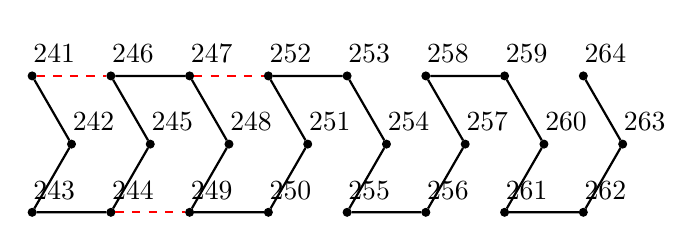
\begin{tikzpicture}[node distance=1cm,every node/.style={draw,circle,fill,inner sep=1pt}]
  \node (3) at (0:0)[label=above right:243]{};
  \node (2) at (60:1)[label=above right:242]{};
  \node (6) at (60:2)[label=above right:246]{};
  
  \node[right of =3](4)[label=above right:244]{};
  \node[right of =4](9)[label=above right:249]{};
  \node[right of =9](10)[label=above right:250]{};
  \node[right of =10](15)[label=above right:255]{};
  \node[right of =15](16)[label=above right:256]{};
  \node[right of =16](21)[label=above right:261]{};
  \node[right of =21](22)[label=above right:262]{};
  
  \node[right of =2](5)[label=above right:245]{};
  \node[right of =5](8)[label=above right:248]{};
  \node[right of =8](11)[label=above right:251]{};
  \node[right of =11](14)[label=above right:254]{};
  \node[right of =14](17)[label=above right:257]{};
  \node[right of =17](20)[label=above right:260]{};
  \node[right of =20](23)[label=above right:263]{};
  
  \node[left of= 6] (1) [label=above right:241]{};
  \node[right of =6](7)[label=above right:247]{};
  \node[right of =7](12)[label=above right:252]{};
  \node[right of =12](13)[label=above right:253]{};
  \node[right of =13](18)[label=above right:258]{};
  \node[right of =18](19)[label=above right:259]{};
  \node[right of =19](24)[label=above right:264]{};
  
  
  \draw[thick](1)--(2)--(3)--(4)--(5)--(6)--(7)--(8)--(9)--(10)--(11)--(12)--(13)--(14)--(15)--(16)--(17)--(18)--(19)--(20)--(21)--(22)--(23)--(24);
  \draw[dashed,thick,red](1)--(6);
  \draw[dashed,thick,red](4)--(9);
  \draw[dashed,thick,red](7)--(12);
  \end{tikzpicture}
  }
  \end{minipage}
  
\begin{minipage}{0.05\hsize}
\ \\
\end{minipage}

%%%%%%%%%%%%%%Dzag-1%%%%%%%%%%%%%%%%%
\begin{minipage}{0.3\hsize}
\centering
\scalebox{0.5}{
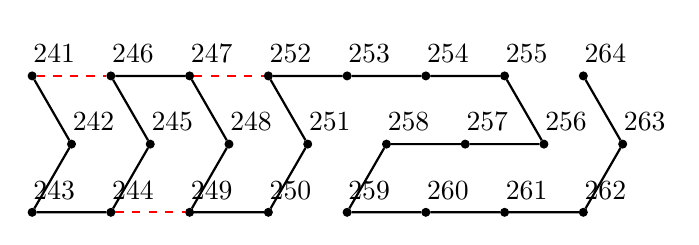
\begin{tikzpicture}[node distance=1cm,every node/.style={draw,circle,fill,inner sep=1pt}]
  \node (3) at (0:0)[label=above right:243]{};
  \node (2) at (60:1)[label=above right:242]{};
  \node (6) at (60:2)[label=above right:246]{};
  
  \node[right of =3](4)[label=above right:244]{};
  \node[right of =4](9)[label=above right:249]{};
  \node[right of =9](10)[label=above right:250]{};
  \node[right of =10](19)[label=above right:259]{};
  \node[right of =19](20)[label=above right:260]{};
  \node[right of =20](21)[label=above right:261]{};
  \node[right of =21](22)[label=above right:262]{};
  
  \node[right of =2](5)[label=above right:245]{};
  \node[right of =5](8)[label=above right:248]{};
  \node[right of =8](11)[label=above right:251]{};
  \node[right of =11](18)[label=above right:258]{};
  \node[right of =18](17)[label=above right:257]{};
  \node[right of =17](16)[label=above right:256]{};
  \node[right of =16](23)[label=above right:263]{};
  
  \node[left of= 6] (1) [label=above right:241]{};
  \node[right of =6](7)[label=above right:247]{};
  \node[right of =7](12)[label=above right:252]{};
  \node[right of =12](13)[label=above right:253]{};
  \node[right of =13](14)[label=above right:254]{};
  \node[right of =14](15)[label=above right:255]{};
  \node[right of =15](24)[label=above right:264]{};
  
  
  \draw[thick](1)--(2)--(3)--(4)--(5)--(6)--(7)--(8)--(9)--(10)--(11)--(12)--(13)--(14)--(15)--(16)--(17)--(18)--(19)--(20)--(21)--(22)--(23)--(24);
  \draw[dashed,thick,red](1)--(6);
  \draw[dashed,thick,red](4)--(9);
  \draw[dashed,thick,red](7)--(12);
  \end{tikzpicture}
  }
  \end{minipage}


  \end{tabular}
  \caption{The possible three conformations of DFAO-zag1: Dzag1-f0, Dzag1-0, and Dzag1-1 from left.}
  \label{fig:DFAO-zag1}
\end{figure} 
%%%%%%%%%%

DFAO-zig1's collaboratively detect the first 0 in two phases.
Phase1 is to copy all the 1's before the first 0 and Phase2 is to copy all the bits after the first 0.
These phases are distinguished by the relative position at which a DFAO-zig1 starts folding to the copier above (in Phase1 it is at the bottom, while in Phase2 it is at the top, as suggested in Figure~\ref{fig:DFAO-zig1}).
In Phase1, DFAO-zig1s certainly take the conformation Dzig1-1 (the top left conformation in Figure~\ref{fig:DFAO-zig1}).
In Phase1, if the half-adder above outputs 0, this is the first 0. 
Then the DFAO-zig1 takes the conformation Dzig1-f0 instead, ending at the top to transition to Phase 2.
Each of the succeeding DFAO-zig1s takes one of the other two conformations Dzig1-20 and Dzig1-21 to copy all the remaining bits. 
Note that there is a cushion between two DFAO-zig1s called \textit{spacer}.
Spacers have been already used to prevent undesirable interference among components.
They are implemented as a glider (see Example~\ref{ex:glider}), hence capable of propagating 1bit on which phase the system is in.
In the first zag, DFAO-zag1's just propagate 0's, 1's, and the first 0 by taking the proper one of the three conformations in Figure~\ref{fig:DFAO-zag1}.

%%%%%%%%%%%%%%%%%%%%%%%%%%%%%%%%%%%%%%%%%%%%
\begin{figure}[h]
\begin{tabular}{c}
%%%%%%%%%%%%Dzig2-1%%%%%%%%%%%%%%%%%
\begin{minipage}{0.3\hsize}
\centering
\scalebox{0.5}{
  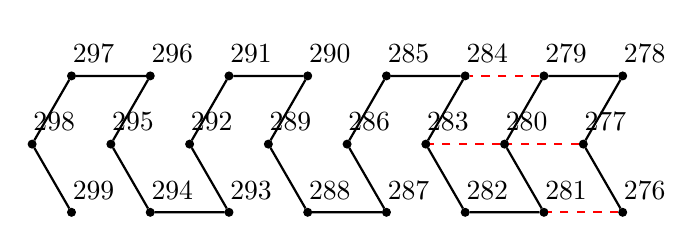
\begin{tikzpicture}[node distance=1cm,every node/.style={draw,circle,fill,inner sep=1pt}]
  \node (1) at (0:0)[label=above right:276]{};
  \node (2) at (120:1)[label=above right:277]{};
  \node (4)at (120:2)[label=above right:279]{};


  \node[right of =4](3)[label=above right:278]{};
  \node[left of =4](9)[label=above right:284]{};
  \node[left of =9](10)[label=above right:285]{};
  \node[left of =10](15)[label=above right:290]{};
  \node[left of =15](16)[label=above right:291]{};
  \node[left of =16](21)[label=above right:296]{};
  \node[left of =21](22)[label=above right:297]{};
  
  \node[left of =2](5)[label=above right:280]{};
  \node[left of =5](8)[label=above right:283]{};
  \node[left of =8](11)[label=above right:286]{};
  \node[left of =11](14)[label=above right:289]{};
  \node[left of =14](17)[label=above right:292]{};
  \node[left of =17](20)[label=above right:295]{};
  \node[left of =20](23)[label=above right:298]{};
  
  \node[left of= 1](6)[label=above right:281]{};
  \node[left of =6](7)[label=above right:282]{};
  \node[left of =7](12)[label=above right:287]{};
  \node[left of =12](13)[label=above right:288]{};
  \node[left of =13](18)[label=above right:293]{};
  \node[left of =18](19)[label=above right:294]{};
  \node[left of =19](24)[label=above right:299]{};
  
  \draw[thick](1)--(2)--(3)--(4)--(5)--(6)--(7)--(8)--(9)--(10)--(11)--(12)--(13)--(14)--(15)--(16)--(17)--(18)--(19)--(20)--(21)--(22)--(23)--(24);
  \draw[dashed,thick,red](1)--(6);
  \draw[dashed,thick,red](2)--(5);
  \draw[dashed,thick,red](5)--(8);
  \draw[dashed,thick,red](4)--(9);
  \end{tikzpicture}
  }
\end{minipage}

\begin{minipage}{0.05\hsize}
\ \\
\end{minipage}

%%%%%%%%%%%%Dzig2-0%%%%%%%%%%%%%%%%%
\begin{minipage}{0.3\hsize}
\centering
\scalebox{0.5}{
  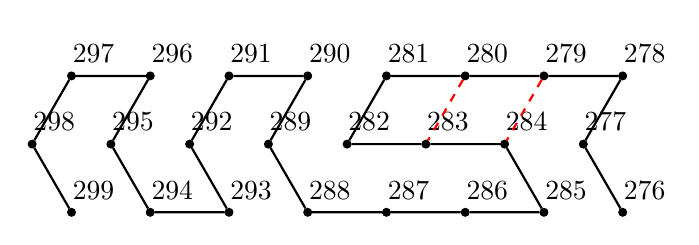
\begin{tikzpicture}[node distance=1cm,every node/.style={draw,circle,fill,inner sep=1pt}]
  \node (1) at (0:0)[label=above right:276]{};
  \node (2) at (120:1)[label=above right:277]{};
  \node (4)at (120:2)[label=above right:279]{};


  \node[right of =4](3)[label=above right:278]{};
  \node[left of =4](5)[label=above right:280]{};
  \node[left of =5](6)[label=above right:281]{};
  \node[left of =6](15)[label=above right:290]{};
  \node[left of =15](16)[label=above right:291]{};
  \node[left of =16](21)[label=above right:296]{};
  \node[left of =21](22)[label=above right:297]{};
  
  \node[left of =2](9)[label=above right:284]{};
  \node[left of =9](8)[label=above right:283]{};
  \node[left of =8](7)[label=above right:282]{};
  \node[left of =7](14)[label=above right:289]{};
  \node[left of =14](17)[label=above right:292]{};
  \node[left of =17](20)[label=above right:295]{};
  \node[left of =20](23)[label=above right:298]{};
  
  \node[left of= 1](10)[label=above right:285]{};
  \node[left of =10](11)[label=above right:286]{};
  \node[left of =11](12)[label=above right:287]{};
  \node[left of =12](13)[label=above right:288]{};
  \node[left of =13](18)[label=above right:293]{};
  \node[left of =18](19)[label=above right:294]{};
  \node[left of =19](24)[label=above right:299]{};
  
  \draw[thick](1)--(2)--(3)--(4)--(5)--(6)--(7)--(8)--(9)--(10)--(11)--(12)--(13)--(14)--(15)--(16)--(17)--(18)--(19)--(20)--(21)--(22)--(23)--(24);

  \draw[dashed,thick,red](5)--(8);
  \draw[dashed,thick,red](4)--(9);
  \end{tikzpicture}
  }
\end{minipage}

\begin{minipage}{0.05\hsize}
\ \\
\end{minipage}

%%%%%%%%%%%%Dzig2-f0%%%%%%%%%%%%%%%%%
\begin{minipage}{0.3\hsize}
\centering
\scalebox{0.5}{
  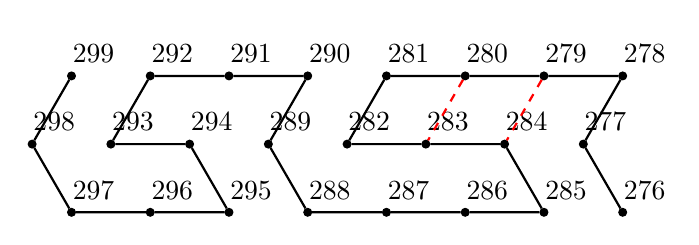
\begin{tikzpicture}[node distance=1cm,every node/.style={draw,circle,fill,inner sep=1pt}]
  \node (1) at (0:0)[label=above right:276]{};
  \node (2) at (120:1)[label=above right:277]{};
  \node (4)at (120:2)[label=above right:279]{};


  \node[right of =4](3)[label=above right:278]{};
  \node[left of =4](5)[label=above right:280]{};
  \node[left of =5](6)[label=above right:281]{};
  \node[left of =6](15)[label=above right:290]{};
  \node[left of =15](16)[label=above right:291]{};
  \node[left of =16](17)[label=above right:292]{};
  \node[left of =17](24)[label=above right:299]{};
  
  \node[left of =2](9)[label=above right:284]{};
  \node[left of =9](8)[label=above right:283]{};
  \node[left of =8](7)[label=above right:282]{};
  \node[left of =7](14)[label=above right:289]{};
  \node[left of =14](19)[label=above right:294]{};
  \node[left of =19](18)[label=above right:293]{};
  \node[left of =18](23)[label=above right:298]{};
  
  \node[left of= 1](10)[label=above right:285]{};
  \node[left of =10](11)[label=above right:286]{};
  \node[left of =11](12)[label=above right:287]{};
  \node[left of =12](13)[label=above right:288]{};
  \node[left of =13](20)[label=above right:295]{};
  \node[left of =20](21)[label=above right:296]{};
  \node[left of =21](22)[label=above right:297]{};
  
  \draw[thick](1)--(2)--(3)--(4)--(5)--(6)--(7)--(8)--(9)--(10)--(11)--(12)--(13)--(14)--(15)--(16)--(17)--(18)--(19)--(20)--(21)--(22)--(23)--(24);

  \draw[dashed,thick,red](5)--(8);
  \draw[dashed,thick,red](4)--(9);
  \end{tikzpicture}
  }
\end{minipage}

 \\
 \\
%%%%%%%%%%%%Dzig2-f00%%%%%%%%%%%%%%%%%
\begin{minipage}{0.4\hsize}
\centering
\scalebox{0.5}{
  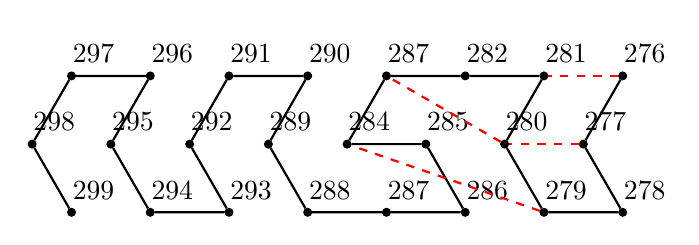
\begin{tikzpicture}[node distance=1cm,every node/.style={draw,circle,fill,inner sep=1pt}]
  \node (3) at (0:0)[label=above right:278]{};
  \node (2) at (120:1)[label=above right:277]{};
  \node (6)at (120:2)[label=above right:281]{};


  \node[left of =3](4)[label=above right:279]{};
  \node[left of =4](11)[label=above right:286]{};
  \node[left of =11](12)[label=above right:287]{};
  \node[left of =12](13)[label=above right:288]{};
  \node[left of =13](18)[label=above right:293]{};
  \node[left of =18](19)[label=above right:294]{};
  \node[left of =19](24)[label=above right:299]{};
  
  \node[left of =2](5)[label=above right:280]{};
  \node[left of =5](10)[label=above right:285]{};
  \node[left of =10](9)[label=above right:284]{};
  \node[left of =9](14)[label=above right:289]{};
  \node[left of =14](17)[label=above right:292]{};
  \node[left of =17](20)[label=above right:295]{};
  \node[left of =20](23)[label=above right:298]{};
    
  \node[right of= 6](1)[label=above right:276]{};
  \node[left of =6](7)[label=above right:282]{};
  \node[left of =7](8)[label=above right:287]{};
  \node[left of =8](15)[label=above right:290]{};
  \node[left of =15](16)[label=above right:291]{};
  \node[left of =16](21)[label=above right:296]{};
  \node[left of =21](22)[label=above right:297]{};
  
  \draw[thick](1)--(2)--(3)--(4)--(5)--(6)--(7)--(8)--(9)--(10)--(11)--(12)--(13)--(14)--(15)--(16)--(17)--(18)--(19)--(20)--(21)--(22)--(23)--(24);
  \draw[dashed,thick,red](1)--(6);
  \draw[dashed,thick,red](2)--(5);
  \draw[dashed,thick,red](5)--(8);
  \draw[dashed,thick,red](4)--(9);
  \end{tikzpicture}
  }
\end{minipage}

\begin{minipage}{0.1\hsize}
\ \\
\end{minipage}

%%%%%%%%%%%%Dzig2-f01%%%%%%%%%%%%%%%%%
\begin{minipage}{0.4\hsize}
\centering
\scalebox{0.5}{
  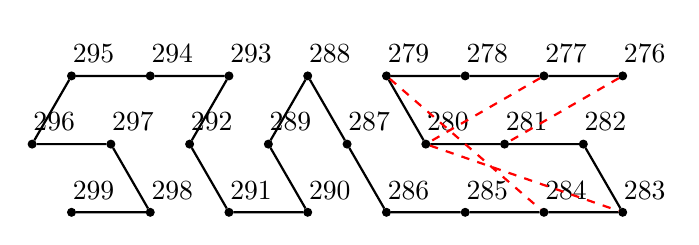
\begin{tikzpicture}[node distance=1cm,every node/.style={draw,circle,fill,inner sep=1pt}]
  \node (8) at (0:0)[label=above right:283]{};
  \node (7) at (120:1)[label=above right:282]{};
  \node (2)at (120:2)[label=above right:277]{};

  \node[left of =8](9)[label=above right:284]{};
  \node[left of =9](10)[label=above right:285]{};
  \node[left of =10](11)[label=above right:286]{};
  \node[left of =11](15)[label=above right:290]{};
  \node[left of =15](16)[label=above right:291]{};
  \node[left of =16](23)[label=above right:298]{};
  \node[left of =23](24)[label=above right:299]{};
  
  \node[left of =7](6)[label=above right:281]{};
  \node[left of =6](5)[label=above right:280]{};
  \node[left of =5](12)[label=above right:287]{};
  \node[left of =12](14)[label=above right:289]{};
  \node[left of =14](17)[label=above right:292]{};
  \node[left of =17](22)[label=above right:297]{};
  \node[left of =22](21)[label=above right:296]{};
    
  \node[right of= 2](1)[label=above right:276]{};
  \node[left of =2](3)[label=above right:278]{};
  \node[left of =3](4)[label=above right:279]{};
  \node[left of =4](13)[label=above right:288]{};
  \node[left of =13](18)[label=above right:293]{};
  \node[left of =18](19)[label=above right:294]{};
  \node[left of =19](20)[label=above right:295]{};
  
  \draw[thick](1)--(2)--(3)--(4)--(5)--(6)--(7)--(8)--(9)--(10)--(11)--(12)--(13)--(14)--(15)--(16)--(17)--(18)--(19)--(20)--(21)--(22)--(23)--(24);
  \draw[dashed,thick,red](1)--(6);
  \draw[dashed,thick,red](2)--(5);
  \draw[dashed,thick,red](5)--(8);
  \draw[dashed,thick,red](4)--(9);
  \end{tikzpicture}
  }
\end{minipage}
  
\end{tabular}

  \caption{The possible five conformations of DFAO-zig2: (top) Dzig2-1, Dzig2-0, Dzig2-f0, (bottom) Dzig2-f00, and Dzig2-f01. }
  \label{fig:DFAO-zig2}
\end{figure} 

%%%%%%%%%%%%%%%%%%%%%%%%%%%%%%%%%%%%%%%%%%%%%%%%
\begin{figure}[h]
\begin{tabular}{c}
%%%%%%%%%%%%%%Dzag2-L0%%%%%%%%%%%%%%%%%
\begin{minipage}{0.3\hsize}
\centering
\scalebox{0.5}{
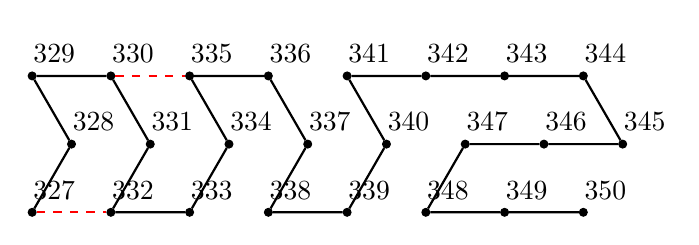
\begin{tikzpicture}[node distance=1cm,every node/.style={draw,circle,fill,inner sep=1pt}]
  \node (1) at (0:0)[label=above right:327]{};
  \node (2) at (60:1)[label=above right:328]{};
  \node (4)at (60:2)[label=above right:330]{};
  
  \node[right of =1](6)[label=above right:332]{};
  \node[right of =6](7)[label=above right:333]{};
  \node[right of =7](12)[label=above right:338]{};
  \node[right of =12](13)[label=above right:339]{};
  \node[right of =13](22)[label=above right:348]{};
  \node[right of =22](23)[label=above right:349]{};
  \node[right of =23](24)[label=above right:350]{};
  
  \node[right of =2](5)[label=above right:331]{};
  \node[right of =5](8)[label=above right:334]{};
  \node[right of =8](11)[label=above right:337]{};
  \node[right of =11](14)[label=above right:340]{};
  \node[right of =14](21)[label=above right:347]{};
  \node[right of =21](20)[label=above right:346]{};
  \node[right of =20](19)[label=above right:345]{};
  
  \node[left of= 4] (3) [label=above right:329]{};
  \node[right of =4](9)[label=above right:335]{};
  \node[right of =9](10)[label=above right:336]{};
  \node[right of =10](15)[label=above right:341]{};
  \node[right of =15](16)[label=above right:342]{};
  \node[right of =16](17)[label=above right:343]{};
  \node[right of =17](18)[label=above right:344]{};
  
  
  \draw[thick](1)--(2)--(3)--(4)--(5)--(6)--(7)--(8)--(9)--(10)--(11)--(12)--(13)--(14)--(15)--(16)--(17)--(18)--(19)--(20)--(21)--(22)--(23)--(24);
  \draw[dashed,thick,red](1)--(6);
  \draw[dashed,thick,red](4)--(9);
  \end{tikzpicture}
  }
  \end{minipage}
  
\begin{minipage}{0.05\hsize}
\ \\
\end{minipage}

%%%%%%%%%%%%%%Dzag2-L1%%%%%%%%%%%%%%%%%
\begin{minipage}{0.3\hsize}
\centering
\scalebox{0.5}{
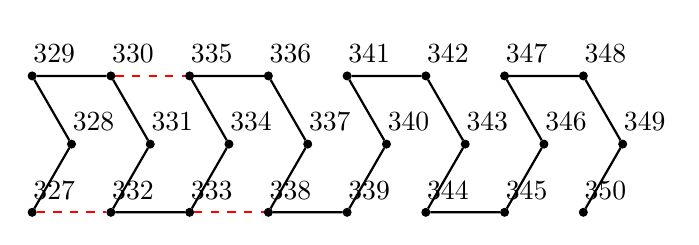
\begin{tikzpicture}[node distance=1cm,every node/.style={draw,circle,fill,inner sep=1pt}]
  \node (1) at (0:0)[label=above right:327]{};
  \node (2) at (60:1)[label=above right:328]{};
  \node (4)at (60:2)[label=above right:330]{};
  
  \node[right of =1](6)[label=above right:332]{};
  \node[right of =6](7)[label=above right:333]{};
  \node[right of =7](12)[label=above right:338]{};
  \node[right of =12](13)[label=above right:339]{};
  \node[right of =13](18)[label=above right:344]{};
  \node[right of =18](19)[label=above right:345]{};
  \node[right of =19](24)[label=above right:350]{};
  
  \node[right of =2](5)[label=above right:331]{};
  \node[right of =5](8)[label=above right:334]{};
  \node[right of =8](11)[label=above right:337]{};
  \node[right of =11](14)[label=above right:340]{};
  \node[right of =14](17)[label=above right:343]{};
  \node[right of =17](20)[label=above right:346]{};
  \node[right of =20](23)[label=above right:349]{};
  
  \node[left of= 4] (3) [label=above right:329]{};
  \node[right of =4](9)[label=above right:335]{};
  \node[right of =9](10)[label=above right:336]{};
  \node[right of =10](15)[label=above right:341]{};
  \node[right of =15](16)[label=above right:342]{};
  \node[right of =16](21)[label=above right:347]{};
  \node[right of =21](22)[label=above right:348]{};
  
  
  \draw[thick](1)--(2)--(3)--(4)--(5)--(6)--(7)--(8)--(9)--(10)--(11)--(12)--(13)--(14)--(15)--(16)--(17)--(18)--(19)--(20)--(21)--(22)--(23)--(24);
  \draw[dashed,thick,red](1)--(6);
  \draw[dashed,thick,red](4)--(9);
  \draw[dashed,thick,red](7)--(12);
  \end{tikzpicture}
  }
  \end{minipage}
  
\begin{minipage}{0.05\hsize}
\ \\
\end{minipage}

%%%%%%%%%%%%%%Dzag2-T1%%%%%%%%%%%%%%%%%
\begin{minipage}{0.3\hsize}
\centering
\scalebox{0.5}{
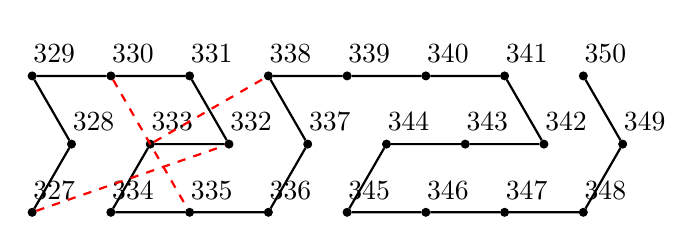
\begin{tikzpicture}[node distance=1cm,every node/.style={draw,circle,fill,inner sep=1pt}]
  \node (1) at (0:0)[label=above right:327]{};
  \node (2) at (60:1)[label=above right:328]{};
  \node (4)at (60:2)[label=above right:330]{};
  
  \node[right of =1](8)[label=above right:334]{};
  \node[right of =8](9)[label=above right:335]{};
  \node[right of =9](10)[label=above right:336]{};
  \node[right of =10](19)[label=above right:345]{};
  \node[right of =19](20)[label=above right:346]{};
  \node[right of =20](21)[label=above right:347]{};
  \node[right of =21](22)[label=above right:348]{};
  
  \node[right of =2](7)[label=above right:333]{};
  \node[right of =7](6)[label=above right:332]{};
  \node[right of =6](11)[label=above right:337]{};
  \node[right of =11](18)[label=above right:344]{};
  \node[right of =18](17)[label=above right:343]{};
  \node[right of =17](16)[label=above right:342]{};
  \node[right of =16](23)[label=above right:349]{};
  
  \node[left of= 4] (3) [label=above right:329]{};
  \node[right of =4](5)[label=above right:331]{};
  \node[right of =5](12)[label=above right:338]{};
  \node[right of =12](13)[label=above right:339]{};
  \node[right of =13](14)[label=above right:340]{};
  \node[right of =14](15)[label=above right:341]{};
  \node[right of =15](24)[label=above right:350]{};
  
  
  \draw[thick](1)--(2)--(3)--(4)--(5)--(6)--(7)--(8)--(9)--(10)--(11)--(12)--(13)--(14)--(15)--(16)--(17)--(18)--(19)--(20)--(21)--(22)--(23)--(24);
  \draw[dashed,thick,red](1)--(6);
  \draw[dashed,thick,red](4)--(9);
  \draw[dashed,thick,red](7)--(12);
  \end{tikzpicture}
  }
  \end{minipage}

\\

%%%%%%%%%%%%%%Dzag-R0%%%%%%%%%%%%%%%%%
\begin{minipage}{0.3\hsize}
\centering
\scalebox{0.5}{
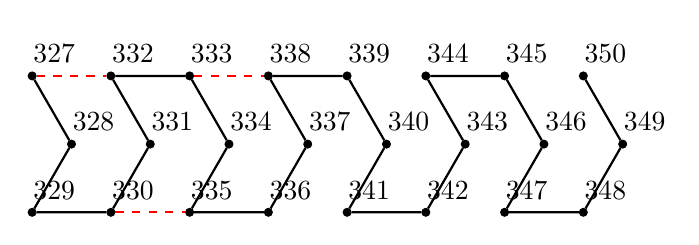
\begin{tikzpicture}[node distance=1cm,every node/.style={draw,circle,fill,inner sep=1pt}]
  \node (3) at (0:0)[label=above right:329]{};
  \node (2) at (60:1)[label=above right:328]{};
  \node (6) at (60:2)[label=above right:332]{};
  
  \node[right of =3](4)[label=above right:330]{};
  \node[right of =4](9)[label=above right:335]{};
  \node[right of =9](10)[label=above right:336]{};
  \node[right of =10](15)[label=above right:341]{};
  \node[right of =15](16)[label=above right:342]{};
  \node[right of =16](21)[label=above right:347]{};
  \node[right of =21](22)[label=above right:348]{};
  
  \node[right of =2](5)[label=above right:331]{};
  \node[right of =5](8)[label=above right:334]{};
  \node[right of =8](11)[label=above right:337]{};
  \node[right of =11](14)[label=above right:340]{};
  \node[right of =14](17)[label=above right:343]{};
  \node[right of =17](20)[label=above right:346]{};
  \node[right of =20](23)[label=above right:349]{};
  
  \node[left of= 6] (1) [label=above right:327]{};
  \node[right of =6](7)[label=above right:333]{};
  \node[right of =7](12)[label=above right:338]{};
  \node[right of =12](13)[label=above right:339]{};
  \node[right of =13](18)[label=above right:344]{};
  \node[right of =18](19)[label=above right:345]{};
  \node[right of =19](24)[label=above right:350]{};
  
  
  \draw[thick](1)--(2)--(3)--(4)--(5)--(6)--(7)--(8)--(9)--(10)--(11)--(12)--(13)--(14)--(15)--(16)--(17)--(18)--(19)--(20)--(21)--(22)--(23)--(24);
  \draw[dashed,thick,red](1)--(6);
  \draw[dashed,thick,red](4)--(9);
  \draw[dashed,thick,red](7)--(12);
  \end{tikzpicture}
  }
  \end{minipage}
  
\begin{minipage}{0.05\hsize}
\ \\
\end{minipage}
%%%%%%%%%%%%%%Dzag-R1%%%%%%%%%%%%%%%%%
\begin{minipage}{0.3\hsize}
\centering
\scalebox{0.5}{
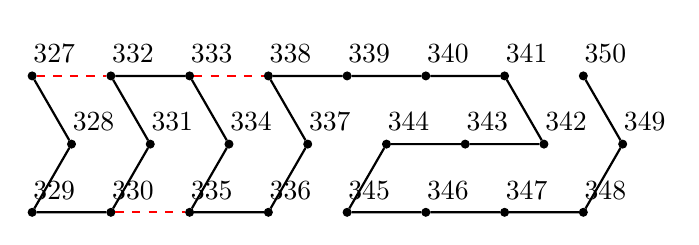
\begin{tikzpicture}[node distance=1cm,every node/.style={draw,circle,fill,inner sep=1pt}]
  \node (3) at (0:0)[label=above right:329]{};
  \node (2) at (60:1)[label=above right:328]{};
  \node (6) at (60:2)[label=above right:332]{};
  
  \node[right of =3](4)[label=above right:330]{};
  \node[right of =4](9)[label=above right:335]{};
  \node[right of =9](10)[label=above right:336]{};
  \node[right of =10](19)[label=above right:345]{};
  \node[right of =19](20)[label=above right:346]{};
  \node[right of =20](21)[label=above right:347]{};
  \node[right of =21](22)[label=above right:348]{};
  
  \node[right of =2](5)[label=above right:331]{};
  \node[right of =5](8)[label=above right:334]{};
  \node[right of =8](11)[label=above right:337]{};
  \node[right of =11](18)[label=above right:344]{};
  \node[right of =18](17)[label=above right:343]{};
  \node[right of =17](16)[label=above right:342]{};
  \node[right of =16](23)[label=above right:349]{};
  
  \node[left of= 6] (1) [label=above right:327]{};
  \node[right of =6](7)[label=above right:333]{};
  \node[right of =7](12)[label=above right:338]{};
  \node[right of =12](13)[label=above right:339]{};
  \node[right of =13](14)[label=above right:340]{};
  \node[right of =14](15)[label=above right:341]{};
  \node[right of =15](24)[label=above right:350]{};
  
  
  \draw[thick](1)--(2)--(3)--(4)--(5)--(6)--(7)--(8)--(9)--(10)--(11)--(12)--(13)--(14)--(15)--(16)--(17)--(18)--(19)--(20)--(21)--(22)--(23)--(24);
  \draw[dashed,thick,red](1)--(6);
  \draw[dashed,thick,red](4)--(9);
  \draw[dashed,thick,red](7)--(12);
  \end{tikzpicture}
  }
  \end{minipage}

  \end{tabular}

  \caption{The possible five conformations of DFAO-zag2: (top) Dzag2-L0, Dzag2-L1, Dzag2-T1, (bottom) Dzag2-R0, and Dzag2-R1.}
  \label{fig:DFAO-zag2}
  \end{figure} 
%%%%%%%%%%%%%%%%%%%%%%%%%%%

In the second zig, DFAO-zig2's check whether the first 0 is followed by 0 or 1, being read from LSB.
They first copy all the 1's up to the first 0 by taking the conformation Dzig2-1 (top left in Figure~\ref{fig:DFAO-zig2}).
The next letter is the first 0, which is distinguished from other 0's by the special conformation Dzag1-f0 of the DFAO-zag1 responsible for the bit, or more precisely, by its marker f0. 
Starting at the bottom and reading 0, the DFAO-zig2 can take two conformations Dzig2-0 and Dzig2-f0.
These conformations share the first half.
The marker f0 folds the second half so as to end at the top, yielding Dzig2-f0. 
The next DFAO-zig2 therefore starts to fold at the top so that it takes one of the two conformations Dzig2-f00 and Dzig2-f01 depending on the bit read.
Recall that reading 1 here is equivalent to transitioning to $q_2$, that is, $P[i] = L$.
Observe that Dzig2-f01 is provided with the marker $q_2$, which lets the DFAO-zag2 component below know $P[i] = L$. 
These conformations end at the bottom.
The remaining 0's and 1's are copied by Dzig2-0 and Dzig2-1, respectively.
The second zag starts at the bottom and copy 0's and 1's by the two conformations Dzag2-L0 and Dzag2-L1 of DFAO-zag2 (top left and center in Figure~\ref{fig:DFAO-zag2}) until a DFAO-zag2 encounters a 1, or more precisely, its marker $q_2$, if any. 
Such DFAO-zag2 takes the special conformation Dzag2-T1 and changes the ending position to the top, letting the remaining DFAO-zag2s rather take Dzag2-R0 and Dzag2-R1 for copying, which end at the top.
As such, the second zag can feed $P[i]$ to PFS as explained before, while propagating the current count $i$.

The third zig lets $P[i]$ go through its AO (or $\overline{\rm AO}$) component to be reinterpreted either as A(cute) or as O(btuse) and propagates the current count $i$.   


%%%%%%%%%%%%%%%%%%%%%%%%%%%%%%%
\subsection{Simulation}
These modules can be checked by simulators on our website.
%%%%%%%%%%%%%%%%%%%%%%%%%%%%%%%


%--------------------------------------------------------
	\section*{Acknowledgements}
%--------------------------------------------------------

We would like to thank Hwee Kim and Aleck Johnsen for their helpful advices and discussions.

%--------------------------------------------------------
%	References
	\bibliographystyle{splncs03}
	\bibliography{oritatami}
%--------------------------------------------------------

%--------------------------------------------------------
	\newpage
	\section*{Appendix}
%--------------------------------------------------------

\begin{figure}[h]
\centering
\begin{minipage}{0.45\linewidth}
\centering
\includegraphics[width=\linewidth]{pic/body-rpx1.png}
\end{minipage}
\begin{minipage}{0.05\linewidth}
\ \\
\end{minipage}
\begin{minipage}{0.45\linewidth}
\centering
\includegraphics[width=\linewidth]{pic/body-lpx1.png}
\end{minipage}
\caption{(Left) The two conformations of body-rpx component. 
(Right) The two conformations of body-lpx1 component.}
\label{fig:body-rpx}
\end{figure}



\end{document}
